\documentclass{article}
\usepackage[top=.5in, bottom=1in, left=0.75in, right=0.75in]{geometry}
\usepackage{graphicx}

\title{Data Mining Program Assignment 2 Report}
\author{Hunter Garrison}
\date{Due: March 21, 2024 @ 11:59PM}

\begin{document}

\maketitle  % This command generates the title, author, and date

\section*{Q1. Evaluation of k-Means over Diverse Datasets}

\subsection*{Part C}
We start with showing the datasets and their respective true clustering.

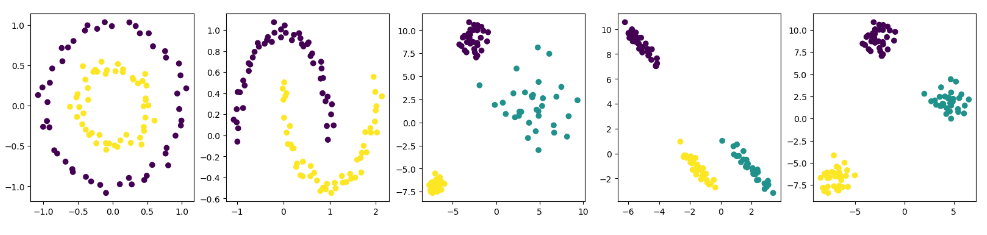
\includegraphics[width=\linewidth]{Images/Screenshot 2024-03-04 174741.png}

Below is a 5 column by 4 row figure of scatter plots where each column pertains to a certain dataset and 
each row pertains to the number of clusters specified in the K-Means algorithm (2, 3, 5, and 10 
respectively).

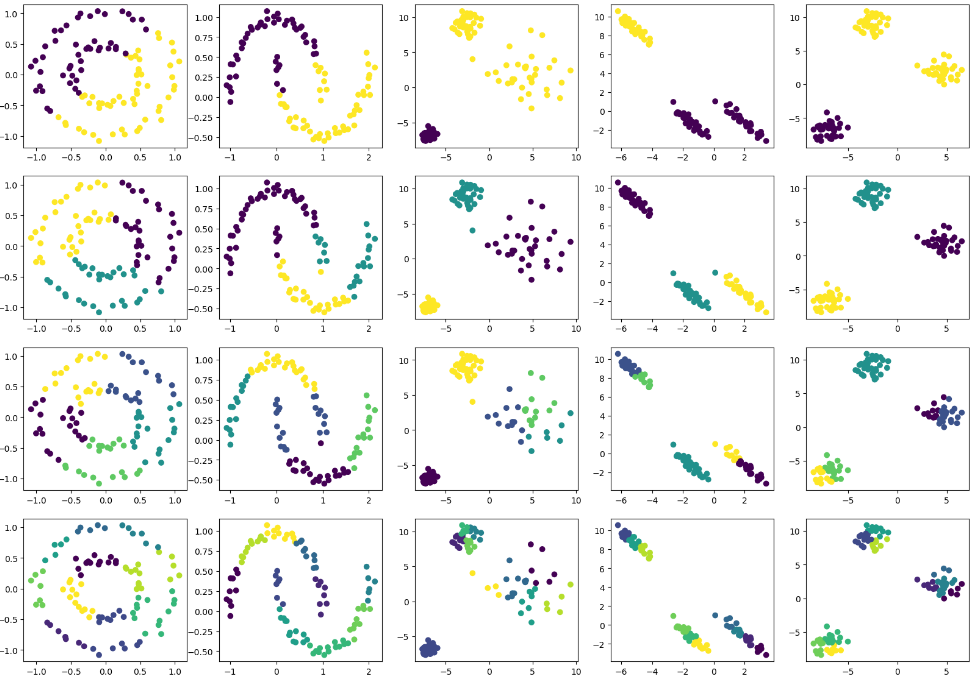
\includegraphics[width=\linewidth]{Images/Screenshot 2024-03-04 175109.png}

We can see that the only dataset in which the K-Means clustering produced correct clusters was for the 
blobs dataset (abbreviated "b" in the coding assignment) with denoted clusters of 3. All other datasets were 
classified incorrectly after using K-Means.

\subsection*{Part D}
Below is a 5 row by 4 column figure where each row pertains to a certain dataset and each column denotes 
specified initial centroids for 2 clusters, random initial centroids for 2 clusters, specified initial 
centroids for 3 clusters, and initial random centroids for 3 clusters, respectively.

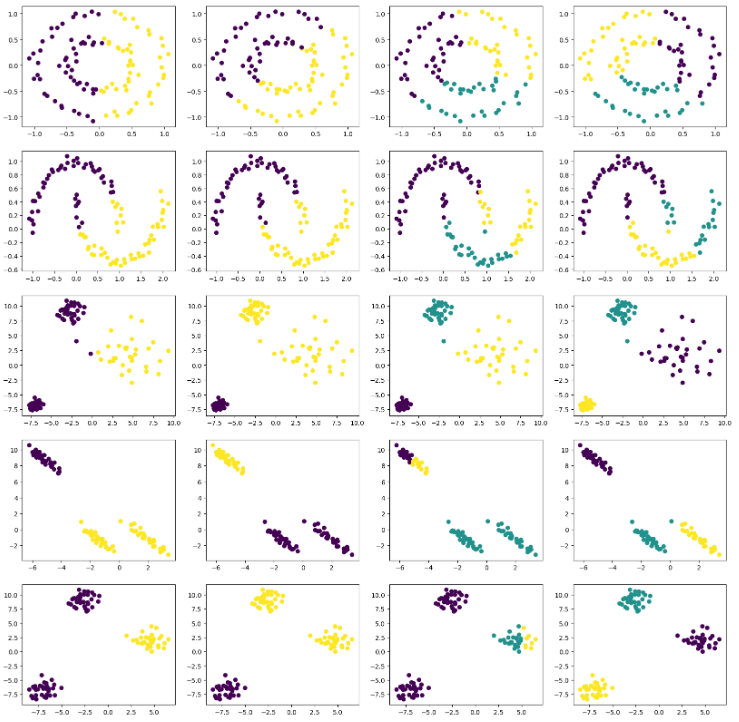
\includegraphics[width=\linewidth]{Images/Screenshot 2024-03-04 175453.png}

We can see that every single dataset is sensitive to the choice of initialization. For the noisy circles, 
our clusters for k=2 start with the division between the clusters to be a diagonal line, but can be changed 
to have the division between the clusters to be a line down the middle (centroids were initialized at 
(0,0) and (1,0)). For the noisy moons, our clusters for k=2 include an extra point in the left cluster 
when we initialize centroids as (0,0) and (1,0). For the blobs with varied variances, when we initialize 
centroids at (0,0) and (1,0) we get the left two clusters merged together whereas random initialization 
merged the left two clusters together. For the anisotropicly distributed data, upon initializing centroids 
at (10,0), (0,0), and (0,0), we end up splitting the top left cluster into two sections. Finally, for the 
blobs we can split the middle right cluster into two sections when initializing centroids at (0,0), (1,0), 
and (2,0).

\section*{Q2. Comparison of Clustering Evaluation Metrics}

\subsection*{Part C}
Below is a plot of SEE as a function of k for k=$1,2,\dots,8$:

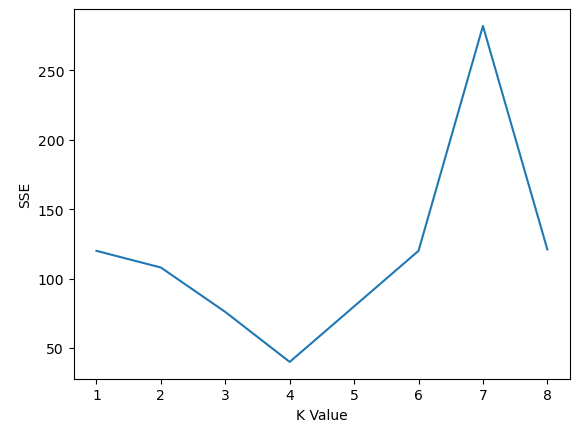
\includegraphics[width=\linewidth]{Images/Screenshot 2024-03-17 164753.png}

According to the elbow method, we want to choose k=4 as our optimal k value.

\subsection*{Part D}
Below is a plot of inertia as a function of k for k=$1,2,\dots,8$:

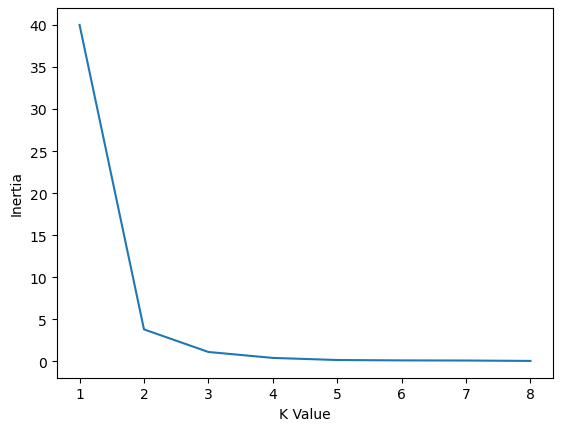
\includegraphics[width=\linewidth]{Images/Screenshot 2024-03-17 165102.png}

Using the elbow method, it looks like k=2 should be our optimal k value, which does not agree with our 
results from 2.C.

\section*{Q3. Hierarchical Clustering}

\subsection*{Part B}
Below is a plot of the dendogram from the hierarchical toy dataset:

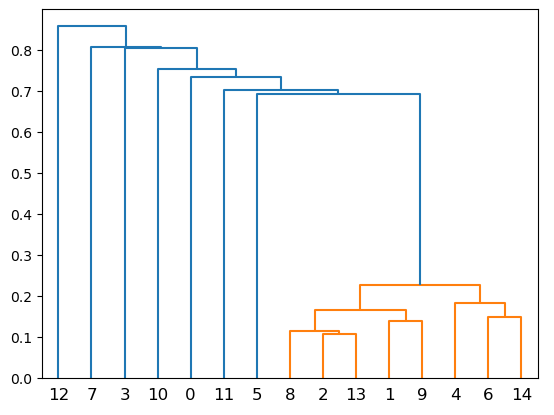
\includegraphics[width=\linewidth]{Images/Screenshot 2024-03-17 165911.png}

\section*{Q4. Evaluation of Hierarchical Clustering over Diverse Datasets}

\subsection*{Part B}
Below is a 5 row by 4 column plot where each row pertains to a specfic dataset and each column pertains to single, 
complete, ward, and centroid linkage type, respectively, using agglomerative clustering:

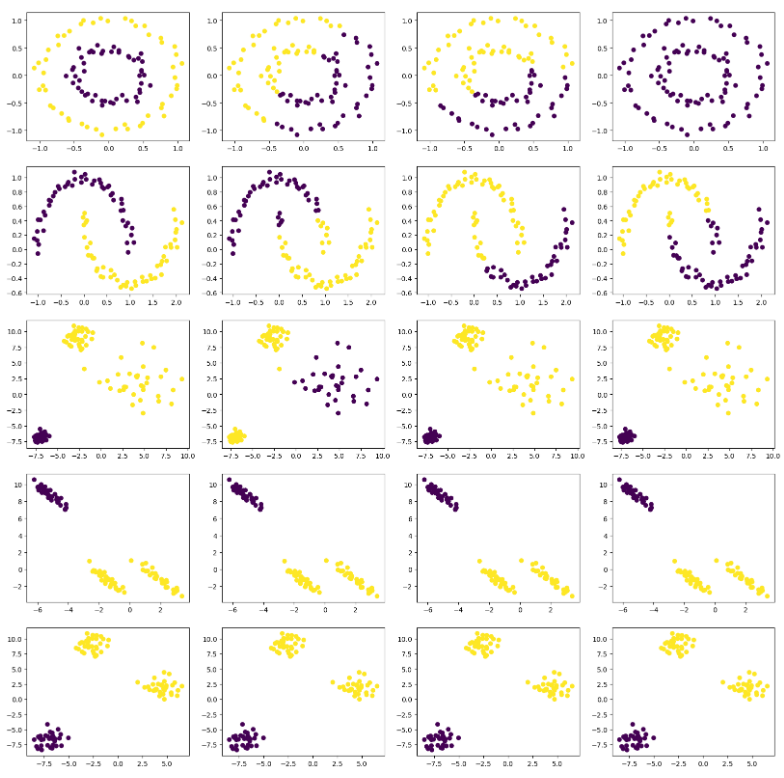
\includegraphics[width=\linewidth]{Images/Screenshot 2024-03-26 083537.png}
The noisy circles and noisy moons datasets are now clustered correctly when using the single linkage type.

\subsection*{Part C}
Below is a 5 row by 4 column plot where each row pertains to a specfic dataset and each column pertains to single, 
complete, ward, and centroid linkage type, respectively, using agglomerative clustering with cut-off distance:

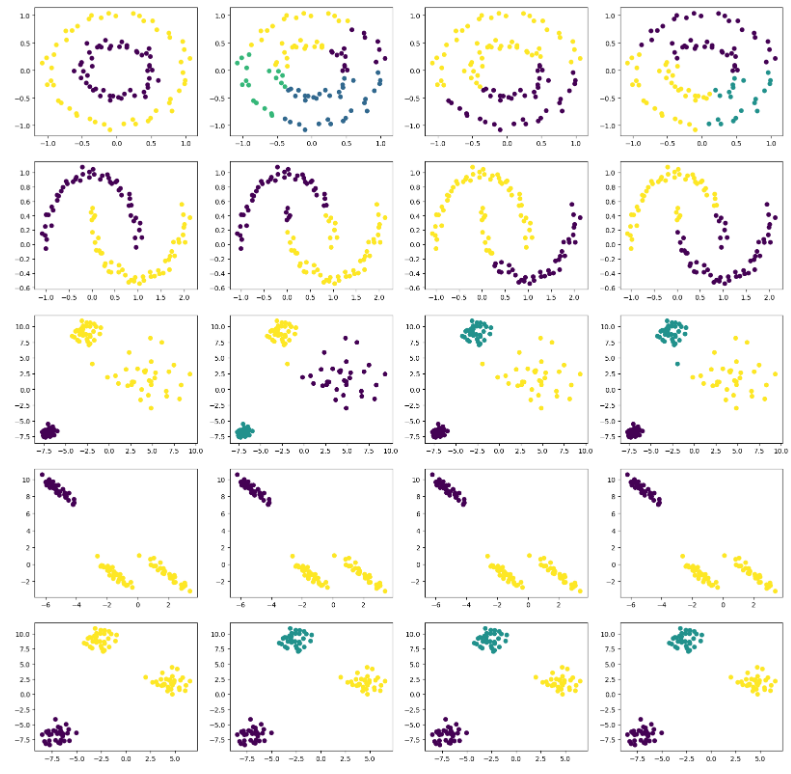
\includegraphics[width=\linewidth]{Images/Screenshot 2024-03-26 083654.png}

We see that we can correctly identify the clusters with each dataset (with varying link types) except for the 
"add" dataset.

\end{document}

